%
\documentclass[preprint,12pt,authoryear]{elsarticle}

%% Use the option review to obtain double line spacing
% \documentclass[authoryear,preprint,review,12pt]{elsarticle}

%% Use the options 1p,twocolumn; 3p; 3p,twocolumn; 5p; or 5p,twocolumn
%% for a journal layout:
%% \documentclass[final,1p,times,authoryear]{elsarticle}
%% \documentclass[final,1p,times,twocolumn,authoryear]{elsarticle}
%% \documentclass[final,3p,times,authoryear]{elsarticle}
%% \documentclass[final,3p,times,twocolumn,authoryear]{elsarticle}
%% \documentclass[final,5p,times,authoryear]{elsarticle}
%% \documentclass[final,5p,times,twocolumn,authoryear]{elsarticle}

%% For including figures, graphicx.sty has been loaded in
%% elsarticle.cls. If you prefer to use the old commands
%% please give \usepackage{epsfig}

%% The amssymb package provides various useful mathematical symbols
\usepackage{amssymb}
%% The amsmath package provides various useful equation environments.
\usepackage{amsmath}
%% The amsthm package provides extended theorem environments
% \usepackage{amsthm}

%% The lineno packages adds line numbers. Start line numbering with
%% \begin{linenumbers}, end it with \end{linenumbers}. Or switch it on
%% for the whole article with \linenumbers.
%% \usepackage{lineno}

\usepackage{array}

\journal{Nuclear Physics B}

\begin{document}

\begin{frontmatter}

%% Title, authors and addresses

%% use the tnoteref command within \title for footnotes;
%% use the tnotetext command for theassociated footnote;
%% use the fnref command within \author or \affiliation for footnotes;
%% use the fntext command for theassociated footnote;
%% use the corref command within \author for corresponding author footnotes;
%% use the cortext command for theassociated footnote;
%% use the ead command for the email address,
%% and the form \ead[url] for the home page:
%% \title{Title\tnoteref{label1}}
%% \tnotetext[label1]{}
%% \author{Name\corref{cor1}\fnref{label2}}
%% \ead{email address}
%% \ead[url]{home page}
%% \fntext[label2]{}
%% \cortext[cor1]{}
%% \affiliation{organization={},
%%            addressline={}, 
%%            city={},
%%            postcode={}, 
%%            state={},
%%            country={}}
%% \fntext[label3]{}

\title{} %% Article title

%% use optional labels to link authors explicitly to addresses:
%% \author[label1,label2]{}
%% \affiliation[label1]{organization={},
%%             addressline={},
%%             city={},
%%             postcode={},
%%             state={},
%%             country={}}
%%
%% \affiliation[label2]{organization={},
%%             addressline={},
%%             city={},
%%             postcode={},
%%             state={},
%%             country={}}

\author{} %% Author name

%% Author affiliation
\affiliation{organization={},%Department and Organization
            addressline={}, 
            city={},
            postcode={}, 
            state={},
            country={}}

%% Abstract
\begin{abstract}
%% Text of abstract
Abstract text.
\end{abstract}

%%Graphical abstract
\begin{graphicalabstract}
%\includegraphics{grabs}
\end{graphicalabstract}

%%Research highlights
\begin{highlights}
\item Research highlight 1
\item Research highlight 2
\end{highlights}

%% Keywords
\begin{keyword}
%% keywords here, in the form: keyword \sep keyword

%% PACS codes here, in the form: \PACS code \sep code

%% MSC codes here, in the form: \MSC code \sep code
%% or \MSC[2008] code \sep code (2000 is the default)

\end{keyword}

\end{frontmatter}

%% Add \usepackage{lineno} before \begin{document} and uncomment 
%% following line to enable line numbers
%% \linenumbers

%% main text
%%

\section{Introduction}\label{sec:introduction}

\subsection{Background and motivation}\label{subsec:background}

The Internet of Things (IoT) has become a foundational element of modern technology, facilitating the development of innovative applications in domains such as smart cities, healthcare, autonomous systems, and other fields. The proliferation of IoT devices has been rapid and significant, with Cisco reporting a global total exceeding 30 billion~\citep{benaboura_comprehensive_nodate}. These devices generate a substantial volume of data, approximately 2 exabytes on a daily basis. Achieving maximum potential from these systems necessitates the implementation of efficient processing and analysis methodologies. This requirement presents a formidable challenge in the domains of data management, resource allocation, and system scalability.

The inherent limitations of IoT devices, such as their small batteries, limited processing power, and minimal storage capacity, render them ill-suited to manage the substantial volumes of data they generate. It is evident that tasks such as real-time processing of sensor data or computation-intensive applications frequently exceed the capabilities of local devices. Conventional approaches entail the delegation of these tasks to centralized cloud servers. However, network limitations and latency sensitivity frequently render this approach inefficient, particularly for real-time applications~\citep{benaboura_comprehensive_nodate}.

In order to address these challenges, fog computing has emerged as a distributed computing paradigm that extends the capabilities of cloud computing to the edge of the network. By facilitating the execution of storage, computation, and data management operations in close proximity to the data source, fog computing contributes to the reduction of latency, power consumption, and network traffic. It is evident that contemporary applications, including but not limited to smart homes, autonomous vehicles, smart agriculture, and healthcare, are contingent on this paradigm in order to satisfy their real-time and location-aware processing requirements as evoked by~\cite{das_review_2023}. Fog computing, first introduced in 2012, provides a hierarchical architecture that serves to bridge the gap between cloud servers and IoT devices, thereby allowing for seamless data flow and operational efficiency~\citep{fahimullah_review_2022}.

Notwithstanding the advantages inherent in task offloading in fog computing, this process is encumbered by numerous challenges. Optimizing resource utilization, reducing energy consumption, and maintaining Quality of Service (QoS) require robust strategies due to the heterogeneous and dynamic nature of fog networks. Factors such as fluctuating workloads, mobility, and task diversity have been identified as contributing to an increase in the complexity of the situation. In order to address these challenges, innovative resource allocation techniques are required, including Machine Learning-based (ML) methods, auction models, and heuristic optimization as~\cite{fahimullah_review_2022} exhibits.

Conventional resource management techniques frequently employ static heuristic approaches, which prove ineffective when confronted with the diverse and dynamic workloads that are characteristic of fog environments. These methods, when configured offline for specific scenarios, lack the scalability and flexibility required for real-time task offloading and resource optimization. Consequently, a substantial decline in performance is experienced as system demands increase~\citep{iftikhar_ai-based_2023}.

To address this problem, metaheuristics such as GA have emerged as powerful optimization techniques capable of handling the multi-objective nature of fog computing task offloading. GAs excel in exploring complex solution spaces and finding near-optimal trade-offs between conflicting objectives such as latency minimization, energy efficiency, and resource utilization. Unlike traditional optimization methods that often focus on single objectives, multi-objective genetic algorithms can simultaneously optimize multiple performance criteria, making them particularly suitable for fog computing environments where various QoS parameters must be balanced. The evolutionary nature of GAs allows them to adapt to dynamic network conditions and heterogeneous resource availability, providing robust solutions for real-time task offloading decisions.

Recent advancements in the field of Artificial Intelligence (AI), particularly deep reinforcement learning (DRL), have demonstrated considerable potential in addressing the intricacies of task offloading in fog environments. Research has demonstrated the efficacy of AI-driven approaches in reducing latency, energy consumption, and operational costs. As~\cite{fahimullah_review_2022} demonstrates in their review, techniques such as centralized Dueling Deep Q-Networks (DDQNs), decentralized learning models, and multi-agent reinforcement learning have been employed to optimize offloading policies and resource allocation. Furthermore, hybrid strategies that integrate artificial intelligence with conventional methods have demonstrated efficacy in heterogeneous fog environments~\citep{mishra_collaborative_2023}.

In order to maintain currency with the latest advancements in this domain, the present study investigates innovative methodologies that integrate the strengths of evolutionary computation and deep reinforcement learning for the purpose of optimizing IoT task offloading. The integration of these approaches addresses the limitations of individual techniques while leveraging their complementary advantages.


\subsection{Contributions}

To address these gaps, this work makes the following key contributions:
\begin{itemize} 
    \item The proposal of a two-transformers-based architecture, utilizing DQRL for the purpose of task offloading within a cloud-fog-edge environment, is hereby presented. The selection of the node (edge, fog or cloud) to execute each incoming task is determined by these models, representing n different ctions. The NOTE system is oriented towards node-level features, such as CPU, buffer, and bandwidth. In contrast, the T-NOTE system incorporates additional task attributes, including size, deadline, and CPU-cycle requirements. This capability facilitates a more precise depiction of the interplay between node resources and task demands within a fog environment.

    \item A transformation of the conventional static genome to a dynamic one is achieved by adapting the Niched Pareto Genetic Algorithm (NPGA) and the Non-dominated Sorting Genetic Algorithm II (NSGA-II), two multi-objective genetic algorithms (GAs), to a MLP as the genome. Subsequently, a comparative analysis was conducted between the GAs and a Deep Q-Learning (DQRL) approach. The implementation of these algorithms in the training of a MLP constitutes a pivotal element of the study. The GA approach is employed in a dynamic setting, thereby enabling the MLP to be optimized for multi-objective offloading in real time.

    
    \item This work also puts forth a model for offloading in hybrid environments that considers a substantial number of parameters for the QoS. To further expand upon the existing body of knowledge, an adaptation of a scenario with a real dataset was implemented within the framework of RayClousSim, which is available at https://github.com/tutur90/Task-Offloading-Fog.


\end{itemize}


\subsection{Paper organization}

The reminder of this paper is structured as follows: Section~\ref{sec:related_work} reviews related work;..................................................... 


\section{Related Work}\label{sec:related_work}


Task offloading in Fog/Cloud environments is a relatively recent research area compared to well-studied domains like image classification or time series forecasting. However, the decision-making process for task offloading is inherently complex due to its combinatorial nature.

\subsection{Deterministic Approaches}
Deterministic algorithms provide a direct method for solving the task offloading problem. For instance, the optimal task assignment algorithm proposed by Yan \textit{et al.}~\cite{yan_optimal_2020} employs a three-step approach: (i) assuming the offloading decisions are pre-determined, (ii) deriving closed-form expressions for optimal offloading, and (iii) implementing bisection search and a one-climb policy. This approach effectively reduces energy consumption and execution time for IoT tasks in Mobile Edge Computing (MEC) systems.

Nevertheless, the task offloading problem is considered NP-hard, as demonstrated in~\cite{guo_algorithmics_2024, jin_task_2024, sarkar_deep_2022}. Consequently, deterministic methods face scalability limitations, prompting the exploration of heuristic, metaheuristic, and AI-based approaches.


\subsection{Heuristic and Metaheuristic Methods}

Heuristic methods are well-suited for scaling in complex edge/cloud environments, as they avoid the exponential computational growth of deterministic algorithms \cite{zhang_survey_2024}. For example, the Deadline and Priority-aware Task Offloading (DPTO) algorithm \cite{adhikari_dpto_2020} schedules tasks by prioritizing delays and task priorities, selecting optimal devices to minimize overall offloading time.

Metaheuristic algorithms, known for their adaptability, have also shown strong performance.~\citep{bernard_dnpga_2024} introduced the Drafting Niched Pareto Genetic Algorithm (D-NPGA), which optimizes task offloading decisions and improves makespan and cost efficiency for IoT tasks in fog/cloud systems.

More sophisticated methods use multiple approaches. For example, Energy-Efficient and Deadline-Aware Task Scheduling in Fog Computing (ETFC) \cite{pakmehr_etfc_2024} employs a Support Vector Machine (SVM) to predict traffic on fog nodes and classify them as low- or high-traffic. Then, they use reinforcement learning (RL) on the low-traffic group and a non-dominated sorting genetic algorithm III (NSGA-III) on the high-traffic group to make the offloading decision. This allows both algorithms to perform better on adequate tasks.

Metaheuristic approaches have gained attention for their ability to address the NP-hard nature of the task offloading problem with flexibility and adaptability. A recent and comprehensive survey by~\cite{rahmani_optimizing_2025} reviewed a wide range of metaheuristic algorithms—including Genetic Algorithms (GA), Particle Swarm Optimization (PSO), Ant Colony Optimization (ACO), and Grey Wolf Optimizer (GWO)—applied to task offloading in IoT environments. The review identified key strengths of these methods in balancing latency, energy consumption, and cost efficiency across heterogeneous fog-edge-cloud infrastructures. Their taxonomy also distinguishes between evolutionary and swarm-based algorithms, showing that hybrid models are increasingly used to adapt to dynamic network conditions. Despite their strengths, the authors noted limitations in scalability and real-time adaptability—areas where AI and deep learning techniques, such as DRL or transformers, may provide an edge.


\subsection{AI Approaches}

Machine learning (ML) has recently demonstrated its efficacy in task offloading. For instance, decision tree classifiers\cite{suryadevara_energy_2021} determine whether tasks should be offloaded to the fog or cloud, resulting in reduced latency and energy consumption. Logistic regression models\cite{bukhari_intelligent_2022} have also been applied, estimating the probability of successful offloading by leveraging maximum likelihood estimation.

Deep learning (DL), a subset of ML, deserves special attention due to its notable advances across various fields. 

Basic deep neural networks (DNNs) have been applied to IoT offloading tasks, such as in\cite{sarkar_deep_2022}, where parallel DNNs optimize cost, energy consumption, and latency. However, deep reinforcement learning (DRL) is often preferred for its decision-making capabilities in dynamic environments.

For example, Jiang \textit{et al.}\cite{jiang_reinforcement_2021} utilized Deep Q-Learning (DQN) to identify optimal offloading policies and resource allocation strategies for user equipment in fog/cloud systems. Their approach combines a dueling deep Q-network for model pre-processing and a distributed deep Q-network for efficient task allocation.

Moreover, multi-agent DRL methods\cite{ren_deep_2021} have been employed to offload IoT tasks. Each IoT device trains its DRL model to select fog access points, followed by a greedy algorithm to determine cloud offloading. This approach demonstrates competitive performance in energy efficiency compared to exhaustive search and genetic algorithms.

Long Short-Term Memory (LSTM) networks, a type of recurrent neural network, are particularly suitable for the temporal dimensions of task offloading. Tu \textit{et al.}\cite{tu_task_2022} combined LSTM with DQN to predict task dynamics in real-time, leveraging observed edge network conditions and server load. This hybrid model significantly improved latency, offloading cost, and task throughput.

Transformers, known for their revolutionary impact on natural language processing (NLP), have also been adapted for task offloading. Gholipour \textit{et al.}\cite{gholipour_tpto_2023} proposed TPTO, a transformer-based framework with Proximal Policy Optimization (PPO). Their model encodes task dependencies using a transformer encoder and employs an actor-critic framework trained with PPO to generate probability distributions for offloading actions, achieving state-of-the-art results in edge computing environments.

While many existing offloading solutions rely on synthetic datasets and focus on Multi-access or Vehicular Edge Computing (MEC/VEC) scenarios~\cite{fahimullah_review_2022, tu_task_2022, gholipour_tpto_2023}, research specifically targeting fog computing remains limited. In particular, models such as Deep Neural Networks (DNNs)~\cite{sarkar_deep_2022} and Deep Q-Learning (DQL)~\cite{jiang_reinforcement_2021} have rarely been evaluated in realistic fog environments using real-world data.

Genetic Algorithms (GAs) are often static in nature, such as in~\cite{bernard_d-npga_2024, pakmehr_etfc_2024}, meaning that they cannot be employed in real-time applications and can only converge through iterations on the same simulation environment where tasks and their order remain static. This characteristic makes them particularly complex to deploy in real-world applications where dynamic adaptation is required.

Transformer-based deep learning techniques remain poorly explored in this domain, despite being state-of-the-art in many fields. Some exploration efforts show promise; however, existing approaches often implement basic action spaces, such as TPTO~\cite{gholipour_tpto_2023}, which is designed with only two actions: offloading the task to the cloud or processing it on the edge.

Algorithms are referenced in the Table~\ref{tab:task_offloading_methods} with the method, the dataset type, the QOS evaluated, and the job type. Used QOS are referenced in the Table~\ref{table:qos_metrics} with their description.


\begin{table*}[h!]\label{tab:task_offloading_methods}
\centering

\resizebox{\textwidth}{!}{%
\begin{tabular}{|l|l|l|l|l|l|l|l|}
\hline
\textbf{Paper} & \textbf{Method} & \textbf{Algorithm} & \textbf{Dataset} & \textbf{QoS} & \textbf{Type of Job} & \textbf{Environment} & \textbf{Tool} \\ \hline
~\cite{yan_optimal_2020} & Deterministic & Optimal Task Assignment & Real & E, ET & IoT tasks & MEC & NA \\ \hline
~\cite{adhikari_dpto_2020} & Heuristic & DPTO & Synthetic & QWT, D & IoT tasks & Cloud \& Fog & NA \\ \hline
~\cite{bernard_d-npga_2024} & Metaheuristic & D-NPGA & Synthetic & C, M & IoT tasks & Cloud \& Fog & Python \\ \hline
This work & Metaheuristic & NPGA/NSGA-II+MLP & Real & C, L, TTR & IoT tasks & Cloud \& Fog & Python, PyTorch \\ \hline
~\cite{pakmehr_etfc_2024} & AI, Metaheuristics & ETFC & C, E, L, DLV & Synthetic & IoT tasks & Fog & NA \\ \hline
~\cite{bukhari_intelligent_2022} & AI & Logistic Regression (LR) & Real & C, E, L & IoT tasks & Cloud \& Fog & Python, Matlab \\ \hline
~\cite{suryadevara_energy_2021} & AI & Decision Tree (DT) & Synthetic & E, L & IoT tasks & Cloud \& Fog & iFogSim \\ \hline
~\cite{sarkar_deep_2022} & AI & Deep Neural Network (DNN) & Synthetic & C, E, L & Mobile & Cloud \& Fog & iFogSim \\ \hline
~\cite{jiang_reinforcement_2021}& AI & Deep Q-Network (DQN) & Synthetic & E, L & Mobile & Cloud \& Fog & Python, Adam optimizer \\ \hline
~\cite{ren_deep_2021} & AI & Multi-agent DRL & Synthetic & E & IoT tasks & Cloud \& Fog & NA \\ \hline
~\cite{tu_task_2022} & AI & DRL+LSTM & Real & C, L, TTR & Mobile & MEC & NA \\ \hline
~\cite{gholipour_tpto_2023} & AI & Transformers PPO & Synthetic & L & IoT tasks & Edge & Python, TensorFlow \\ \hline
This work & AI & DQRL+MLP & Real & C, L, TTR & IoT tasks & Cloud \& Fog & Python, PyTorch \\ \hline
This work & AI & Transformers & Real & C, L, TTR & IoT tasks & Cloud \& Fog & Python, PyTorch \\ \hline
\end{tabular}
}
\caption{Summary of Task Offloading Methods in Fog and Edge Computing}
\end{table*}


\begin{table*}[h]\label{table:qos_metrics}
\centering
\resizebox{\textwidth}{!}{%
\begin{tabular}{ |c|l| }
\hline
\textbf{Metric} & \textbf{Description} \\ \hline
C\@: Cost & Refers to the expenses incurred in task offloading, including computation, storage, and data transfer costs. \\ \hline
L\@: Latency & The time delay between the initiation of a request and the reception of the response. Crucial for real-time applications. \\ \hline
E\@: Energy & The total energy consumed during task offloading, including device and network-level energy usage. \\ \hline
ET\@: Execution Time & The total time taken to execute a task from start to finish, including computation and communication time. \\ \hline
D\@: Delay & The time difference between task submission and the start of its processing. Includes network and processing delays. \\ \hline
M\@: Makespan & The total time required to complete all tasks in a batch or workflow. Indicates overall system efficiency. \\ \hline
QWT\@: Queue Waiting Time & The duration a task spends waiting in the queue before being processed. Impacts response time and throughput. \\ \hline
TTR\@: Task Throw Rate & The rate at which tasks are successfully processed and completed in the system, indicating system throughput. \\ \hline
DLV\@: Dead Line Violation & The percentage or rate of tasks that succeed to complete within their specified deadlines, indicating system reliability and quality of service. \\ \hline
\end{tabular}
}
\caption{Explanation of QoS Metrics in Edge-Fog-Cloud Computing}
\end{table*}


\section{Problem Modeling}
\label{sec:problem_modeling}

\subsection{Scenario Modeling}
\label{sec:problem_modeling}

This scenario is modeled according to foundational concepts presented in\cite{aazam_cloud_2022, bukhari_intelligent_2022, jazayeri_autonomous_2021}, following a three-tier offloading approach that involves \textit{edge}, \textit{fog}, and \textit{cloud} nodes. In Figure~\ref{fig:cloud-architecture}, a high-level cloud-enabled architecture is shown, where a Global Gateway (GG) collects tasks from various IoT devices before determining whether to process them locally or offload them to fog or cloud resources.


A real-world dataset of IoT-generated tasks, is employed to study and evaluate these offloading decisions. The tasks in this dataset vary in size, deadline constraints, and computational complexity, thereby reflecting the heterogeneous nature of practical IoT workloads.

\begin{figure}[ht]
    \centering
    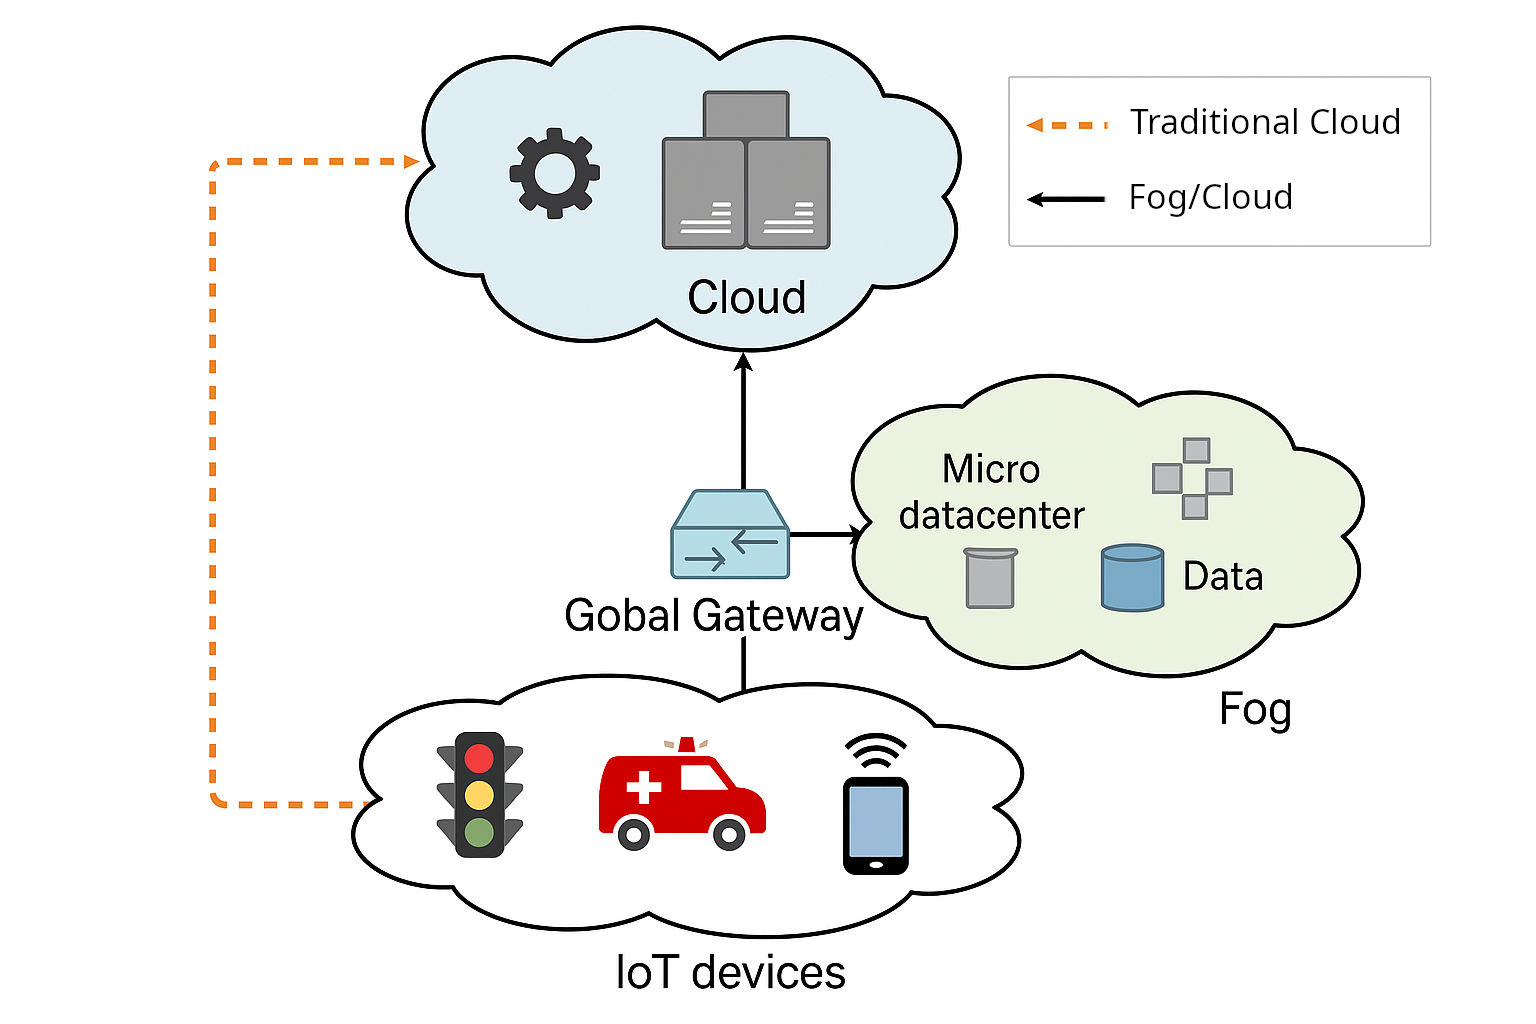
\includegraphics[width=0.75\linewidth]{figs/cloud_architecture.png}
    \caption{System Architecture}
    \label{fig:cloud-architecture}
\end{figure}


\subsubsection{Architecture}
\label{subsec:architecture}

In Figure~\ref{fig:cloud-architecture}, a schematic overview of the \textbf{proposed three-tier architecture} is illustrated. The system is composed of IoT devices (sensors, mobile nodes, and other edge devices) that generate tasks. These tasks subsequently reach the Global Gateway, which processes them locally if resources are available, or decides to offload them to the fog or the cloud based on resource availability and energy considerations.



\paragraph{Global Gateway}
\label{subsubsec:GG}

The GG layer is located at the edge and aggregates tasks from local IoT devices. In addition to routing capabilities, the GG has limited computational power, enabling it to handle \emph{smaller tasks} locally and thus reduce network traffic. This approach is particularly advantageous for time-sensitive tasks that can be processed quickly on-site.

Upon receiving a task, several factors are evaluated:
\begin{itemize}
    \item Node state: The current load on the GG, along with the availability of fog and cloud nodes.
    \item Network conditions: Bandwidth, potential congestion, and latency to fog or cloud nodes.
    \item Energy usage: A predictive assessment of energy costs if the task is executed locally versus offloaded.
    \item Task requirements: Size, computational complexity, and deadline or QoS constraints.
\end{itemize}

A subsequent decision is made to determine the optimal execution strategy for the task. The system evaluates three primary options: processing the task locally if it is computationally feasible and resource-efficient, offloading the task to a nearby Fog Node to leverage edge computing capabilities, or offloading the task directly to a Cloud Node for intensive computational requirements that exceed local and fog node capacities.


\paragraph{Fog Nodes}
\label{subsubsec:Fog}
Fog nodes provide moderate computational resources that exceed those of edge devices but remain below the capacity of cloud data centers. These intermediate computing nodes offer lower latency than distant cloud nodes due to their closer physical proximity to the network edge. Fog nodes serve as an essential intermediate tier for tasks that cannot be processed locally at the Gateway (GG) yet do not require the extensive resources of the cloud infrastructure. This positioning makes them ideal for applications requiring balanced performance between computational capability and response time.

\paragraph{Cloud Nodes}
\label{subsubsec:Cloud}
Cloud nodes represent large-scale data centers with substantial computational and storage capabilities. Although they typically have higher baseline latencies because of greater network distances, they are well suited for computationally intensive applications. Cloud nodes excel in handling large tasks that demand significant CPU and memory resources, making them optimal for complex analytical workloads. They are particularly effective for batch processing scenarios with relaxed real-time constraints, where throughput is prioritized over immediate response. Furthermore, cloud data centers can accommodate high concurrency situations through dynamic resource scaling, allowing them to adapt to varying computational demands efficiently. concurrency situations, as cloud data centers can scale resources dynamically.


CPU capacity: Cloud servers can support a high volume of CPU cycles, facilitating efficient offloading for tasks with elevated computational demands.

\subsection{QoS Modeling}\label{sec:simulation_modeling}

Task offloading decisions are evaluated within the RayCloudSim framework developed by~\cite{zhang2022osttd}, a comprehensive simulation platform for modeling and assessing cloud-edge-IoT computing environments based on LEAF~\citep{WiesnerThamsen_LEAF_2021}.

\subsubsection{Task Throw Rate}\label{subsubsec:task_throw_rate}

In distributed environments, task execution failures can occur due to issues such as \emph{network disconnections}, \emph{node isolation}, or \emph{buffer overflows}.

The \emph{task throw rate} \(\tau\) is defined as:
\begin{equation}
\tau = \frac{\text{Number of failed tasks}}{\text{Total tasks generated}}.
\end{equation}
A lower throw rate is indicative of a more robust and efficient offloading strategy.





























%% Use figure environment to create figures
%% Refer following link for more details.
%% https://en.wikibooks.org/wiki/LaTeX/Floats,_Figures_and_Captions
\begin{figure}[t]%% placement specifier
%% Use \includegraphics command to insert graphic files. Place graphics files in 
%% working directory.
\centering%% For centre alignment of image.
\includegraphics{example-image-a}
%% Use \caption command for figure caption and label.
\caption{Figure Caption}\label{fig1}
%% https://en.wikibooks.org/wiki/LaTeX/Importing_Graphics#Importing_external_graphics
\end{figure}


%% The Appendices part is started with the command \appendix;
%% appendix sections are then done as normal sections
\appendix
\section{Example Appendix Section}\label{app1}

Appendix text.

%% For citations use: 
%%      \citet{<label>} ==> Lamport (1994)
%%       \citep{<label>} ==> (Lamport, 1994)
%%
\citep{mishra_collaborative_2023}
Example citation, See \citet{mishra_collaborative_2023}.

%% If you have bib database file and want bibtex to generate the
%% bibitems, please use
%%
 \bibliographystyle{elsarticle-harv} 
 \bibliography{references}

%% else use the following coding to input the bibitems directly in the
%% TeX file.

%% Refer following link for more details about bibliography and citations.
%% https://en.wikibooks.org/wiki/LaTeX/Bibliography_Management

% \begin{thebibliography}{00}

% %% For authoryear reference style
% % \bibitem[Author(year)]{label}
% % Text of bibliographic item

% \bibitem[Lamport(1994)]{lamport94}
%   Leslie Lamport,
%   \textit{\LaTeX: a document preparation system},
%   Addison Wesley, Massachusetts,
%   2nd edition,
%   1994.

% \end{thebibliography}
\end{document}

\endinput
%%
%% End of file `elsarticle-template-harv.tex'.


